%!TEX root = ../../thesis.tex

\section{Distribution of Exoplanets}

Exoplanetary detections have challenged the theoretical formation models with their variety and distribution of sizes, locations For instance, the discovery of the hot-Jupiter class (large mass planets on close in orbits) challenged the accepted planet formation theories at the time~\citep[.e.g][]{pollack_formation_1996, boss_giant_1997} in which our Solar System was thought to be typical with small rocky planets close to the Sun and large giant planets further away.


The precise characterization of more exoplanets with the detection of exoplanetary atmospheres will allow for the constraints of exoplanetary composition and formation mechanisms to be improved.
For instance, the core accretion model has been able to reproduce the large number of Super-Earths, the correlation be star metallicity and planet frequency~\citep[e.g.][]{santos_spectroscopic_2004, fischer_planetmetallicity_2005}, and the presence of many Hot-Jupiter and Neptune in close-in orbits, with the help of migration mechanisms~\citep[e.g.][]{Triaud_exoplanets_2016}.
Recent models also combine both planetary formation and evolution to describe the observed exoplanets~\citep[e.g.][]{mordasini_characterization_2012} and can reproduce general population properties in a statistically significant way~\citep{mordasini_characterization_2009}.

A proxy for the composition and structure of an exoplanet is the average density, computed from the mass and radius.
A mass-radius diagram is shown in \fref{fig:santerne2018} for Earth-like rocky planets.
The tracks show contours of mass-radius for different theoretical compositions~\citep{brugger_constraints_2017}, while the circles indicate a number of detected small mass exoplanets, with {K2-229\,b} being a Super-Earth with a Mercury-like density~\cite{santerne_earthsized_2018}.
The density can give an approximate composition but for a given mass there are an infinite combinations of metal/silicate/ice and gas that can produce the same radii~\citep[e.g.][]{seager_massradius_2007}.
Low mass planets tend to be rocky and tend to have small or no atmosphere. With rock being in-compressible, to first order, it is relatively insensitive to the incident flux.
The radii of solid exoplanets are sensitive to gas content of the atmosphere as small increase in \ce{H}/\ce{He} can cause a large increase in radius~\citep{adams_ocean_2008}.

When the gas component becomes dominate  planets begin to have radii independent of their mass~\citep[e.g.][]{lopez_understanding_2014}.
The atmospheres of gas giants are also susceptible to stellar irradiation, with close in Hot-Jupiters having inflated atmospheres and larger radii \citep[e.g][]{fortney 2009}. \todo{ Down to here}

\begin{figure}
    \centering
    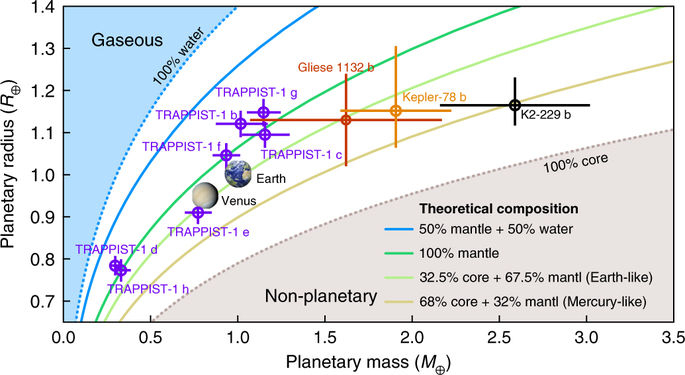
\includegraphics[width=0.7\linewidth]{figures/introduction/santerne_2018}
    \caption{Mass-Radius diagram for rocky planets with composition contours. Adapted from \citet{santerne_earthsized_2018}}
    \label{fig:santerne2018}
\end{figure}



Models for the mass-radius relation are important as they enable insight into the likely planetary properties when only either mass or radius can or has been measured.
For example \citet{chen_probabilistic_2016} develop a probabilistic model over 9 orders-of-magnitude in mass an 3 orders-of-magnitude in radius.
Their model is shown in \fref{fig:mass_radius_relation}.
It shows ... 4 regions with a split at ... fitted to the data ...

 has been explored out to low-mass stars distribution has been extended out to low-mass stars. 



Brown Dwarfs bridge the gap between low-mass stars and giant planets with masses around \(13-80~\textrm{M}_{jup} \)~\citep{chabrier_theory_2000}, 



Recently, there has been a renewed interest in BD candidates triggered by exoplanetary searches.
While several works found similar properties on the two populations, like a similar density~\citep{hatzes_definition_2015}, others have found intriguing differences.
One of the most recent is the different host metallicity of the Brown Dwarf and giant planet populations~\citep{santos_observational_2017, schlaufman_evidence_2018}, a very strong hint of different formation mechanisms.


Extending the Mass-Radius diagram from low mass planets out to low-mass stars in \fref{fig:mass_radius_relation} reveals interesting situation~\citet{chen_probabilistic_2016}.

There are 4 different regions in which the slow of the M-R diagram is different, potential indicating different formation features with the locations of shle indicating different transition boundaries. \textbf{reread paper} 

\begin{figure}[t]
    \centering
    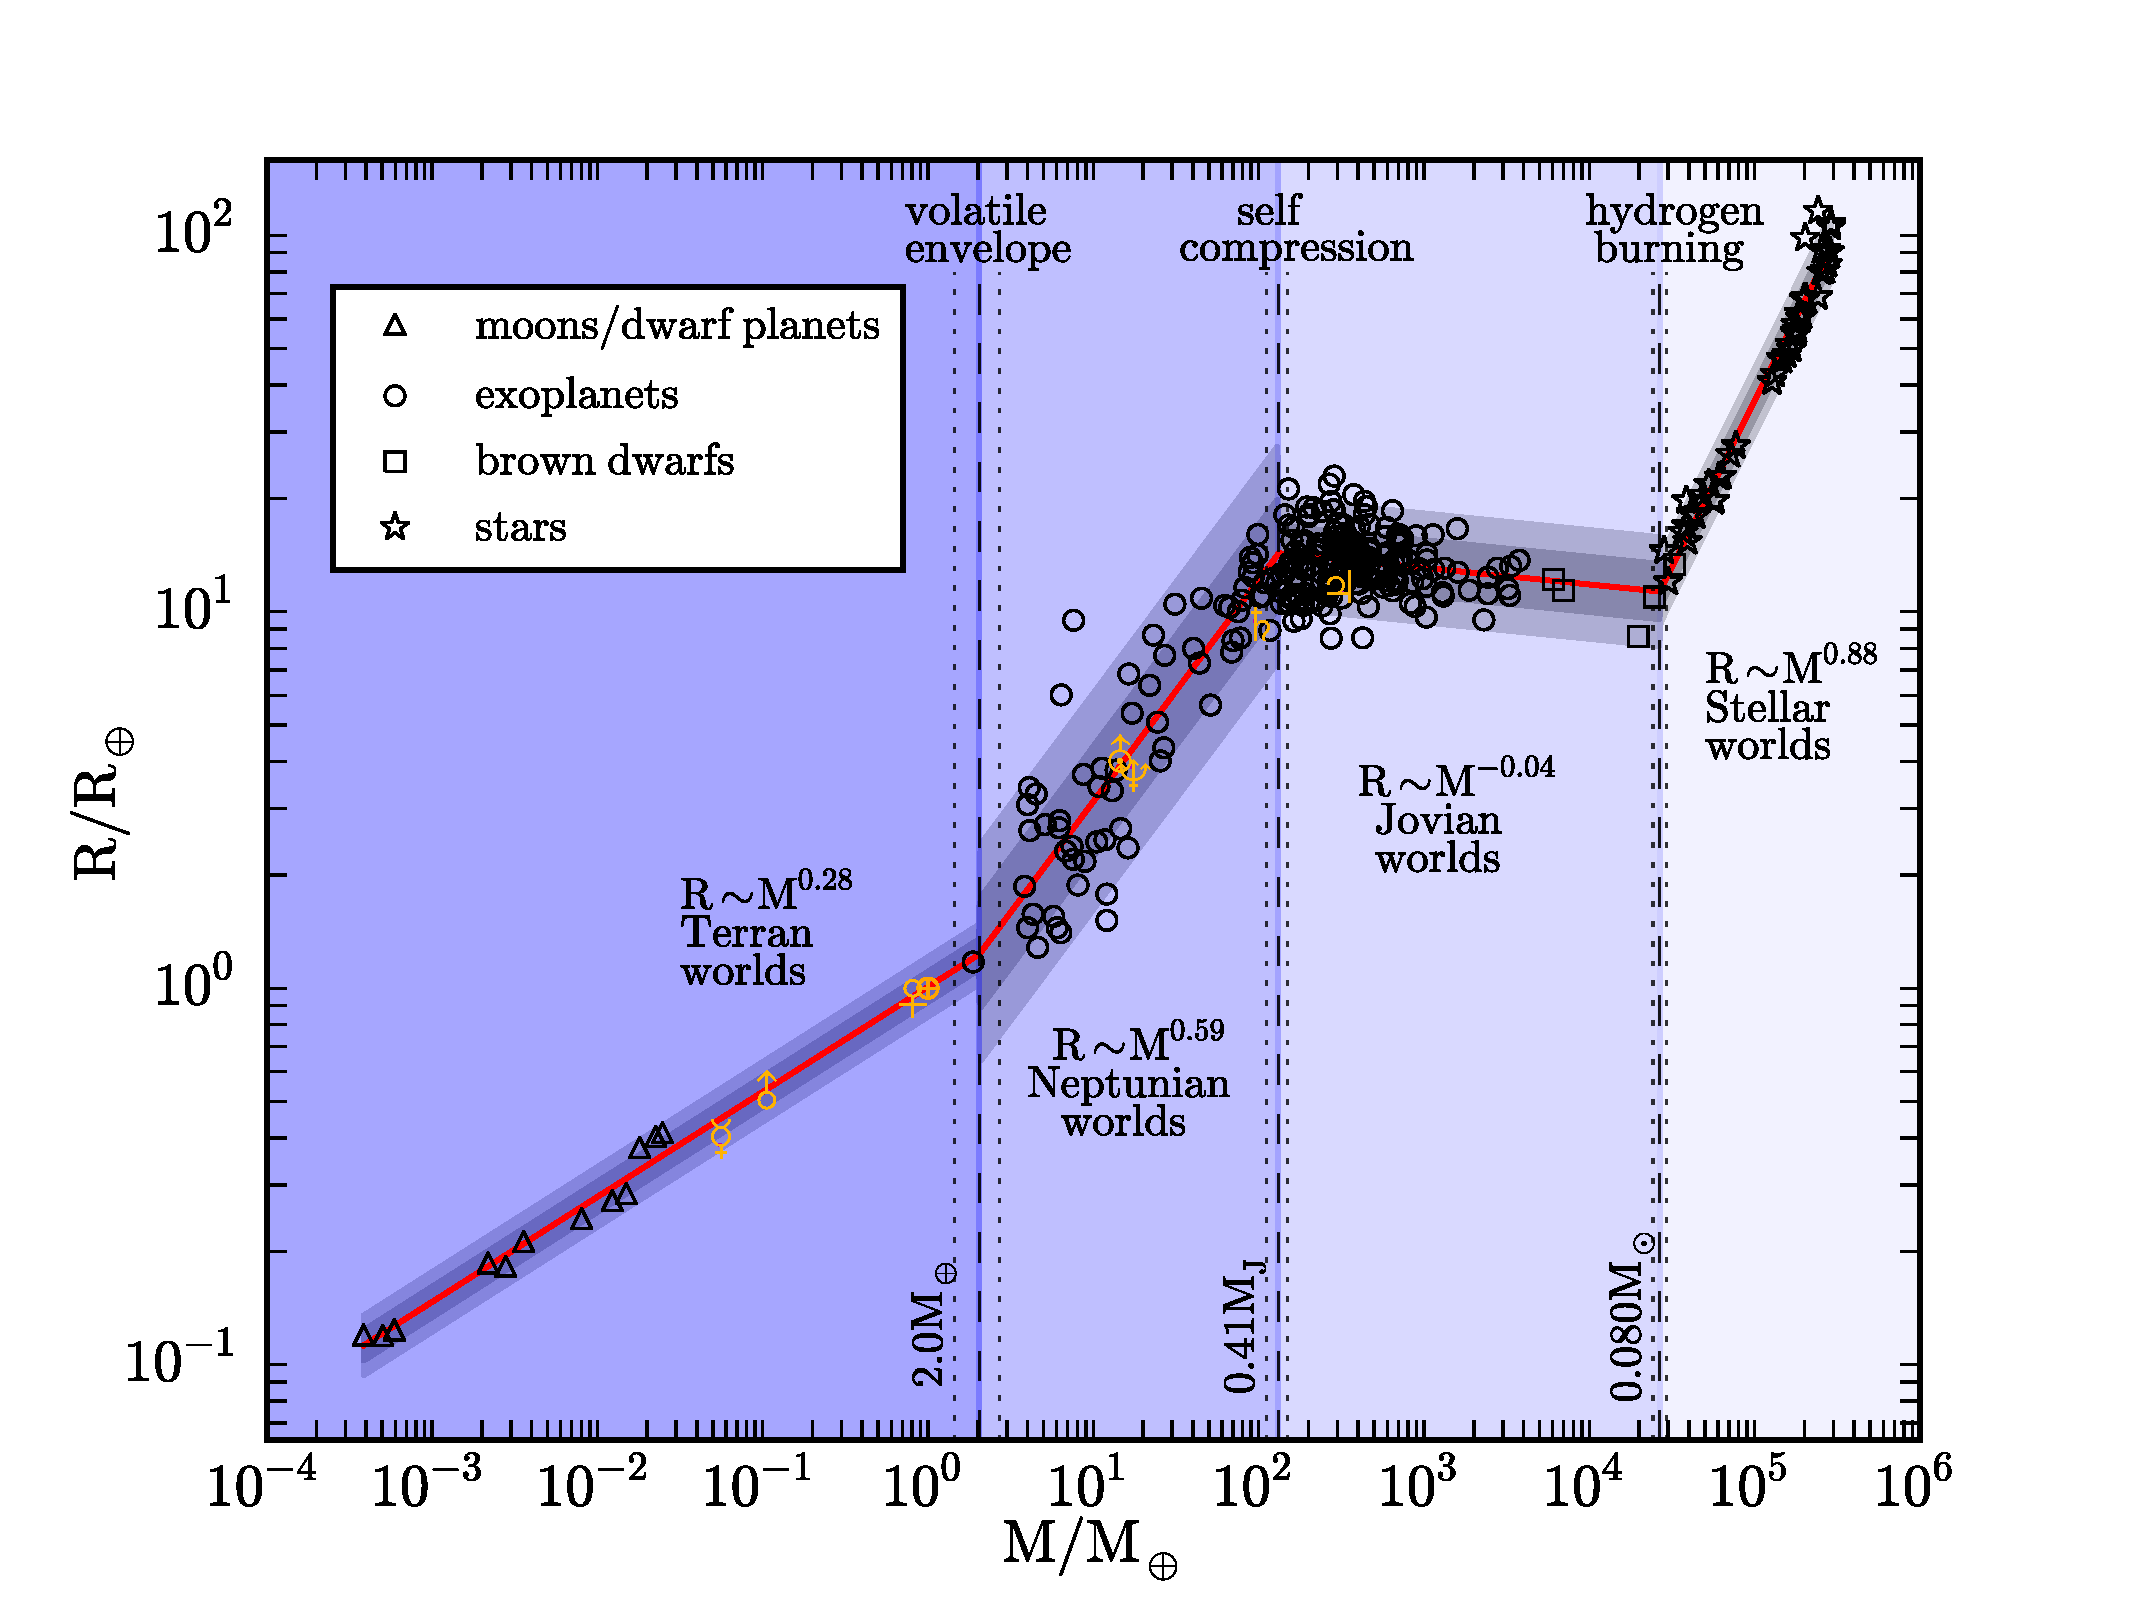
\includegraphics[width=0.9\linewidth]{./figures/introduction/mass_radius_relation.pdf}  \\
    \caption{Left: Mass-Radius relationship from planets to stars~\citet{chen_probabilistic_2016}.}
    \label{fig:mass_radius_relation}
\end{figure}


\citep{santos_observational_2017} Santos et al 2017 \todo{read and quote}  Observational evidence for two distinct giant planet populations





double peak histogram from an {RV} paper?? Faria 2018?


did they form from the molecular cloud when the star was forming or from the remnants of the disk after the star formed like exoplanets....?






\textbf{brown dwarf dessert explore \citet{ranc_moa2007blg197_2015}}


\subsection{Brown Dwarfs}
\todo{This is mainly from the paper still.}
Brown dwarfs (BDs) are sub-stellar objects unable to achieve hydrogen fusion, with masses around \(13-80~\textrm{M}_{jup} \)~\citep{chabrier_theory_2000}, bridging the gap between low-mass stars and giant planets.
Without sustained fusion, brown-dwarfs cool down over time with an age-dependent cooling rate.
Therefore, there is an inherent degeneracy between the mass, age and luminosity of a given BD~\citep{burrows_nongray_1997}.
This degeneracy may be resolved by the observation of several parameters, for instance when a BD is in a binary system with a main sequence host star, using both the host stars age and the masses derived from the dynamical motion.

A paucity of BD companions exists in short period orbits around Sun-like stars (\(\lesssim5 \)\AU), compared to stellar or planetary companions, termed the \emph{brown dwarf desert}~\citep{halbwachs_exploring_2000, zucker_analysis_2001, sahlmann_search_2011}.
As the number of known BDs orbiting solar type stars is low, the characterization of benchmark BDs in the brown dwarf desert~\citep[e.g.][]{crepp_trends_2016} is beneficial in understanding this sub-stellar population and to help constrain formation and evolution theories~\citep{whitworth_formation_2007}.
The BD desert also provides a greater challenge as it reduces the amount of good BD candidates to study.

BDs in binary systems, unlike free-floating BDs, allow for the determination of their masses, when complemented with radial velocity ({RV}) and astrometry measurements.
The {RV} technique provides the mass lower-limit (\mtwosini{}) of binary and planetary companions, while complementary astrometry measurements can often provide mass upper-limits~\citep[e.g.][]{sahlmann_search_2011}.
Measuring or tightening the constraints of BD masses improves the understanding of mass dependence on BD formation processes.
For instance, there is growing evidence that the larger giant planets and BD companions do not follow the well known metallicity-giant planet correlation seen in main-sequence stars with planets~\citep[e.g.][]{santos_spectroscopic_2004,santos_observational_2017, maldonado_searching_2017}.
Photometry along with stellar evolution models~\citep[e.g.][]{baraffe_evolutionary_2003,allard_btsettl_2013} can also be used to estimate the mass of BD companions~\citep[e.g.][]{moutou_eccentricity_2017} if there is sufficient orbital separation, and a precise determination of the age~\citep{soderblom_ages_2010}.




%
%\begin{figure}[t]
%    \centering
%    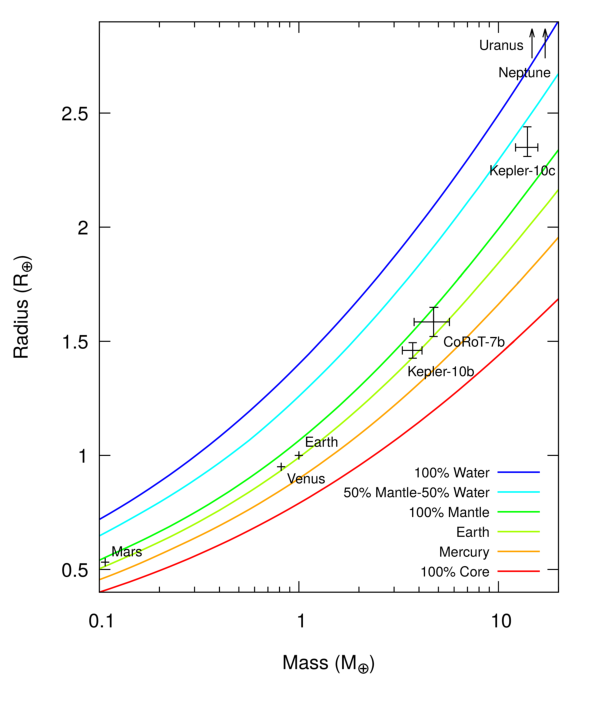
\includegraphics[width=0.4\linewidth]{./figures/introduction/Mass_radius_relation-compostion_Brugger_2017.pdf}
%    \caption{Mass-Radius relationship for (super) Earth-like planets with composition contours.
%        Adapted from~\citet{brugger_constraints_2017}}
%    \label{fig:mass_radius_relation_composition}
%\end{figure}



\begin{figure}
    \centering
    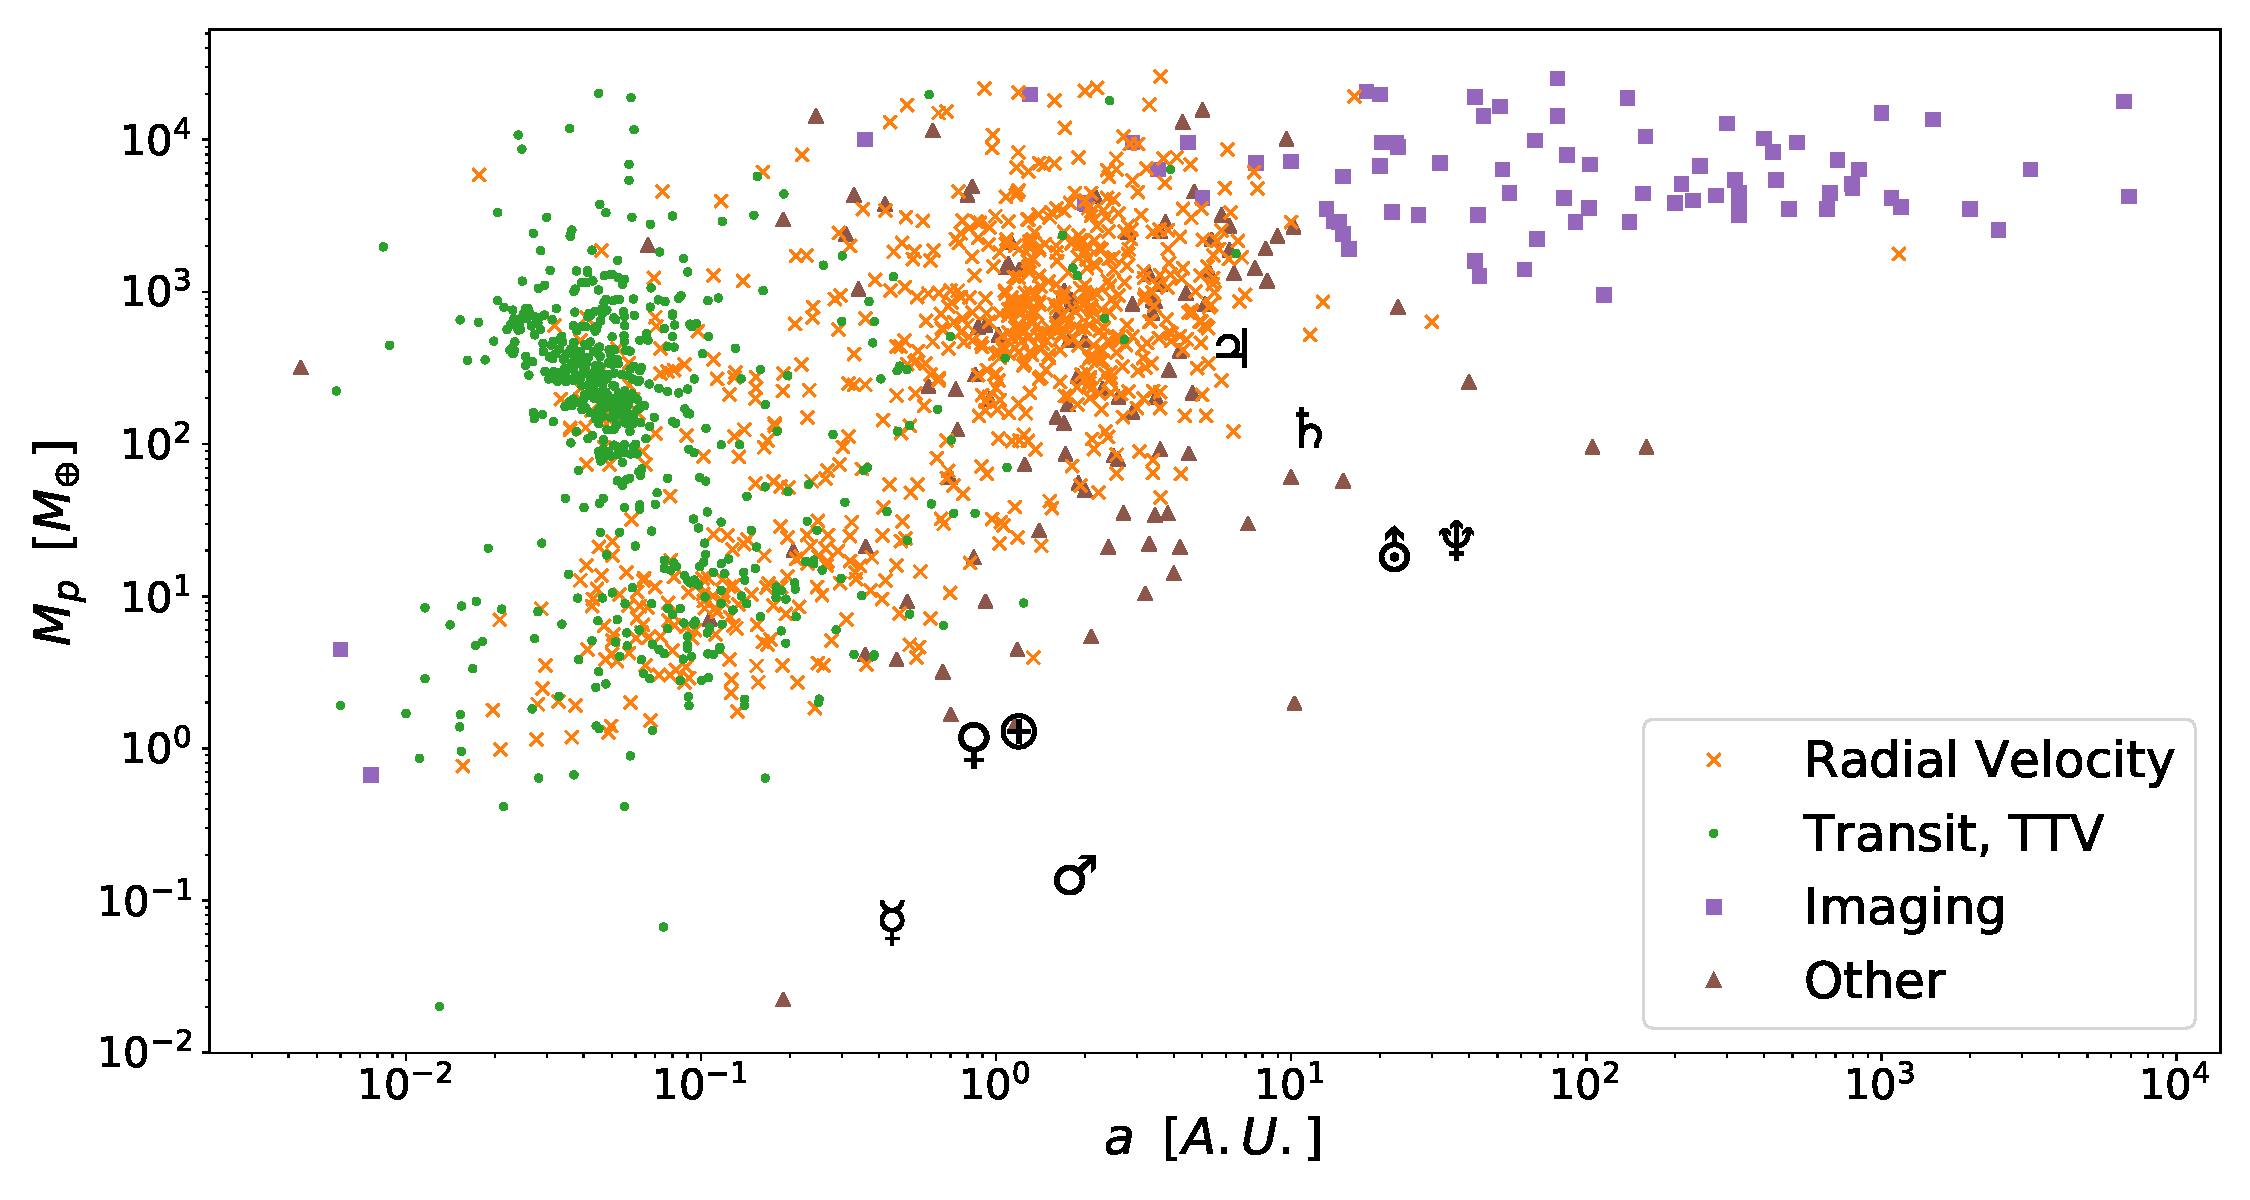
\includegraphics[width=0.\linewidth]{./figures/introduction/exoplanetEU_a_mass.pdf}
    \caption{Eoplanet semi-major axis verses mass diagram.
        The symbols indicate the location of the solar system planets, $\mercury$-Mercury, $\venus$-Venus, $\earth$-Earth, $\mars$-Mars, $\jupiter$-Jupiter, $\saturn$-Saturn, $\uranus$-Uranus, $\neptune$-Neptune.
        Data from \href{http://ww.exoplanet.eu}{exoplanet.eu} October 2018}
    \label{fig:pltoverlayadd}
\end{figure}


Explore what these method have found with exoplanet populations.
